\documentclass[10pt,conference]{IEEEtran}
\usepackage{cite}
\usepackage{float}
\usepackage{minted}
\usepackage[T1]{fontenc}
\usepackage[utf8]{inputenc}
\ifCLASSINFOpdf
   \usepackage[pdftex]{graphicx}
   \graphicspath{{figs/}}
   \DeclareGraphicsExtensions{.pdf,.jpeg,.png}
\else
   \usepackage[dvips]{graphicx}
   \graphicspath{{../figs/}}
   \DeclareGraphicsExtensions{.eps}
\fi
\usepackage[cmex10]{amsmath}
\interdisplaylinepenalty=2500
\usepackage{amsthm}
\newtheorem{definition}{Definition}
\usepackage{algorithmic}
\usepackage{array}
\ifCLASSOPTIONcompsoc
  \usepackage[caption=false,font=normalsize,labelfont=sf,textfont=sf]{subfig}
\else
  \usepackage[caption=false,font=footnotesize]{subfig}
\fi
\usepackage{url}
\hyphenation{op-tical net-works semi-conduc-tor}
\usepackage[left=1.6cm,top=4cm,right=1.6cm,bottom=1.5cm,headheight=1cm]{geometry}
\usepackage{lipsum}
\usepackage{graphicx}
% utilizado para calcular o tamanho da pagina
\usepackage{tikz}
\usepackage{fancyhdr}
\usepackage{tikzpagenodes}
\renewcommand{\headrulewidth}{0pt}
\renewcommand{\footrulewidth}{0pt}
\usetikzlibrary{calc}
\pagestyle{fancy}
\setlength\headheight{12.0pt}
\addtolength{\textheight}{-42.0pt}
\addtolength{\topmargin}{-2.0pt}

\fancyhead[L]{\begin{tikzpicture}[remember picture,overlay]
\draw  let \p1=($(current page.north)-(current page header area.south)$),
      \n1={veclen(\x1,\y1)} in
node [inner sep=0,outer sep=0,below right] 
      at (current page.north west){
\includegraphics[width=\paperwidth,height=\n1]{headerimg.png}};
\end{tikzpicture}}

\fancyfoot[R]{\begin{tikzpicture}[remember picture,overlay]
\draw  let \p1=($(current page footer area.north)-(current page.south)$),
      \n1={veclen(\x1,\y1)} in
node [inner sep=0,outer sep=0,above right] 
      at (current page.south west){
\includegraphics[width=\paperwidth,height=\n1]{footerimg.png}};
\end{tikzpicture}}

\begin{document}
\title{Uso de IA Multimodal para Detecção de Achados em Mamografias com o Modelo MedGEMMA}
\newif\iffinal
\finaltrue
\iffinal
    % \author{
    % \IEEEauthorblockN{Vinicius Tessele}
    % \IEEEauthorblockA{Dept. of Artificial Intelligence \\
    % Biopark Educação \\
    % Toledo, Brazil \\
    % ORCID: 0000-0002-0662-9200}
    % \and
    % \IEEEauthorblockN{Claudio Honorio da Silva Junior}
    % \IEEEauthorblockA{Dept. of Artificial Intelligence \\
    % Biopark Educação \\
    % Toledo, Brazil \\
    % ORCID: 0009-0000-5043-0517}
    % \and
    % \IEEEauthorblockN{Angelo Gabriel}
    % \IEEEauthorblockA{Dept. of Artificial Intelligence \\
    % Biopark Educação \\
    % Toledo, Brazil \\
    % ORCID: 0009-0005-7939-5301}
    % \and
    % \IEEEauthorblockN{Leonardo Tampelini}
    % \IEEEauthorblockA{Dept. of Artificial Intelligence \\
    % Biopark Educação \\
    % Toledo, Brazil \\
    % ORCID: 0009-0000-9307-4444}
    % }
\else
  \author{ID do artigo Latin.science 2020: \cmtid \\ }
\fi
\maketitle
\thispagestyle{fancy}

\begin{abstract}
This study investigates the use of multimodal artificial intelligence (AI) as a clinical decision support tool, with a focus on the detection of findings in mammography. The research employs Google MedGEMMA 4B-IT, an advanced architecture that integrates a medical image encoder (MedSigLIP) with a language model trained to interpret complex clinical descriptions and terminology. Using a real dataset of mammographic images and their corresponding radiology reports, the study evaluates the model's ability to correlate visual and textual information with accurate BI-RADS classification. By analyzing both the model's strengths and its limitations, this work aims to demonstrate the potential of AI to enhance diagnostic precision and efficiency, while reinforcing that it is not a substitute for expert medical judgment. Furthermore, the results provide insights for future supervised fine-tuning efforts, with the goal of improving sensitivity in high-risk categories and reducing false positives.
\end{abstract}

\renewcommand{\IEEEkeywordsname}{Keywords}
\begin{IEEEkeywords}
Multimodal Artificial Intelligence; Medical Imaging; MedGemma 4B-IT.
\end{IEEEkeywords}

\renewcommand{\abstractname}{Resumo}

\begin{abstract}
 O presente estudo investiga o uso da inteligência artificial (IA) multimodal como ferramenta de apoio ao diagnóstico clínico, com ênfase na detecção de achados em mamografias. Para isso, utiliza-se o modelo Google MedGEMMA 4B-IT, uma arquitetura avançada que integra um encoder de imagens médicas (MedSigLIP) com um modelo de linguagem treinado para interpretar terminologia e descrições clínicas complexas. A pesquisa baseia-se em um conjunto real de mamografias e respectivos laudos clínicos, avaliando a capacidade do modelo em associar informações visuais e textuais à classificação correta segundo o sistema BI-RADS. Ao analisar os acertos e limitações da IA, o estudo busca evidenciar seu potencial de apoio à tomada de decisão médica, contribuindo para o desenvolvimento de soluções mais precisas, rápidas e contextualmente informadas, sem substituir o papel essencial da análise humana especializada. Além disso, os resultados fornecem subsídios para futuras etapas de fine-tuning supervisionado, visando aprimorar a sensibilidade do modelo para categorias críticas e reduzir falsos positivos.
\end{abstract}

\renewcommand\IEEEkeywordsname{Palavras-chave}

\begin{IEEEkeywords}
Inteligência Artificial Multimodal; Imagens Médicas; MedGemma 4B-IT.
\end{IEEEkeywords}

\IEEEpeerreviewmaketitle

\section{Introdução} 
O sistema de saúde utiliza recursos e equipamentos tecnológicos de ponta para diagnóstico e tratamento. Esses recursos podem ser integrados com a Inteligência Artificial (IA), de modo a contribuir ainda mais para o diagnóstico precoce de doenças graves, como o câncer de mama. Esses equipamentos têm gerado uma quantidade enorme de dados médicos, incluindo exames de imagem (como mamografias, tomografias e ressonâncias) e registros textuais (como laudos, prontuários e anotações clínicas). Diante desse volume de dados, o uso da IA torna-se cada vez mais promissor. A IA tem grande potencial em aplicações na saúde, mas seu treinamento e implantação enfrentam desafios devido a diversidade dos dados, à complexidade das tarefas e a necessidade de garantir a privacidade dos pacientes\cite{sellergren2025medgemma}.

Modelos capazes de interpretar simultaneamente diferentes modalidades de informação são conhecidos como modelos multimodais. A IA multimodal em saúde representa um avanço significativo por permitir a interpretação conjunta de imagens e textos médicos, potencializando o diagnóstico, que passa a considerar não apenas a imagem, mas também as informações relatadas nos prontuários clínicos.

Esse tipo de modelo não visa substituir a interpretação do médico, mas sim atuar como um assistente inteligente, automatizando tarefas e auxiliando na identificação de achados relevantes que poderiam passar despercebidos.

Este estudo aborda o uso do Google MedGemma 4B-IT, que surge como uma alternativa promissora. Trata-se de um modelo multimodal com 4 bilhões de parâmetros, que combina um encoder de imagens adaptado para a medicina com um modelo de linguagem otimizado para compreender descrições clínicas. O modelo foi treinado com bases de dados anonimizadas, e sua arquitetura multimodal permite flexibilidade para atuar com diversos formatos, inclusive respondendo a perguntas com base em laudos e imagens simultaneamente.


\begin{figure}[!h]
\centering
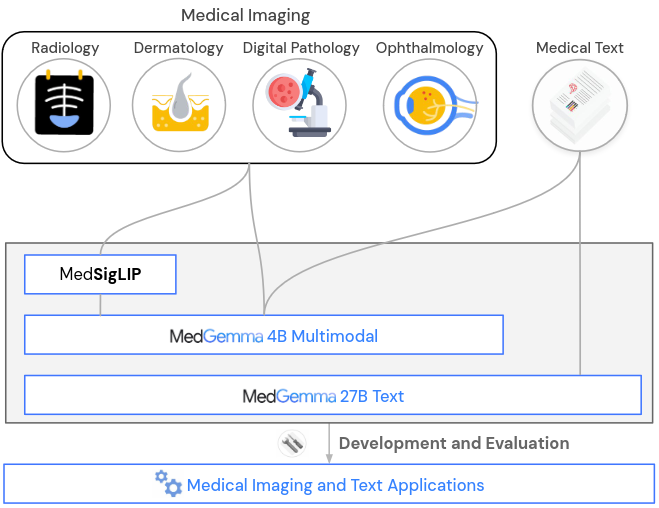
\includegraphics[width=3.5in]{figs/med.png}
\caption{Medical Imaging}
\label{fig:med}
\end{figure}

O objetivo principal deste trabalho é avaliar o desempenho do modelo Google MedGemma 4B-IT em tarefas de identificação de achados clínicos em mamografias, utilizando um conjunto real de imagens e laudos médicos. Além disso, discutimos o potencial do modelo, suas aplicações e limitações.

Fig.~\ref{fig:med}. Visão geral MedGemma, destacando o encoder de imagens MedSigLIP, o MedGemma 4B Multimodal e o MedGemma 27B Text. Adaptado de Sellergren et al. (2025).

A Fig.~\ref{fig:med} apresenta a arquitetura geral da coleção de modelos MedGemma, composta por variantes textuais e multimodais, com o encoder de imagens MedSigLIP integrado ao MedGemma 4B-IT.



\section{Referencia Teorico}
A neoplasia mamária resulta do crescimento descontrolado de células nas mamas, podendo ser classificada como benigna ou maligna. Quando maligna, é conhecida como câncer de mama, é o tipo de câncer mais comum entre mulheres em muitas regiões do mundo \cite{inca2025}. No Brasil, desconsiderando os casos de tumores de pele não melanoma, o câncer de mama é o tipo de câncer mais frequente entre mulheres em todas as regiões, apresentando maior incidência nas regiões Sul e Sudeste. Estima-se que, a cada ano do período de 2023 a 2025, ocorram 73.610 novos casos, correspondendo a uma taxa ajustada de incidência de 41,89 casos por 100.000 mulheres \cite{inca2025}. A detecção precoce do câncer de mama é essencial para melhorar as taxas de sobrevivência e possibilita o tratamento menos agressivo \cite{paulinelli2004diagnostico}. A mamografia é um exame de imagem, que permite a detecção de lesões de forma antecipada. No entanto enfrenta desafios, como a limitada sensibilidade em casos de tecidos mamários densos bem como erros interpretativos. \cite{guerreiro2024ia}. A fim de padronizar a interpretação dos exames de imagem das mamas, foi desenvolvido o sistema BI-RADS (Breast Imaging Reporting and Data System), este sistema classifica os achados mamográficos em categorias numeradas de 0 a 6, cada uma associada a um nível de risco para malignidade e uma conduda clínica recomenda. Com essa padronização auxilia não somente a comunicação entre radiologistas e médicos, mas também orienta o manejo clínico.

\begin{table}[!h]
\renewcommand{\arraystretch}{1.3}
\caption{Classificação BI-RADS}
\label{table:birads}
\centering
\begin{tabular}{|c|l|p{2.5cm}|}
\hline
\textbf{Categoria} & \textbf{Descrição} & \textbf{Conduta} \\
\hline
0 & Inconclusivo & Exames adicionais (mamografia, US ou RM complementar) \\
\hline
1 & Negativo & Rastreamento normal \\
\hline
2 & Achado benigno & Rastreamento normal \\
\hline
3 & Provavelmente benigno & Controle por imagem em 6 meses \\
\hline
4 & Suspeita de malignidade & Biópsia recomendada \\
\hline
5 & Altamente sugestiva de malignidade & Biópsia urgente \\
\hline
6 & Malignidade confirmada & Acompanhamento e planejamento terapêutico \\
\hline
\end{tabular}

\vspace{0.2cm}
\small \textbf{Fonte:} Adaptado de Magny et al. (2023), *StatPearls – NCBI*; Weerakkody et al. (2025), Radiopaedia.org \cite{weerakkody2025birads}.
\end{table}

A inteligência artificial (IA), vem oferecendo inúmeras aplicações no diagnóstico médicos utilizando algoritmos sofisticados capaz de processar grandes quantidade de dados proveniente das imagens de mamografia de forma rápida.

Os algortimos de IA, especialemente os de aprendizado profundo, demonstram capacidade de processar grandes volumes de dados, com velocidade e precisão superiores a métodos convencionais \cite{hosny2018ai}.

Em especial a radiologia mamária, os sistemas de IA foram na análise isolada de imagens, utilizando redes neurais convolucionais, para identificar padrões visuais. Contudo essa abordagem pode ser complementada com informações textuais disponívies nos laudos médicos, histórico clínicos dos pacientes, que são fundamentais para o fechamento do diagnóstico clínico completo.

Os modelos multimodais surgem para que se integre simultaneamente diferentes tipos de dados (Imagem, Texto), para uma análise mais abrangente e contextualizada. Segundo Simon et al. \cite{simon2025multimodal}, "modelos de IA multimodal podem combinar tanto imagens quanto metadados clínicos, e estão rapidamente se tornando uma abordagem popular integrada ao ecossistema médico". Ainda assim, é fundamental que a validação final dos achados continue sendo realizada por profissionais médicos.

Os modelos de Linguagem Grandes (LLMs) constituem um componente essencial dessa arquitetura multimodal. Estes modelos, baseados em arquiteturas de transformers, são capazes de compreender e gerar texto de forma contextualmente relevante, podendo interpretar descrições clínicas complexas e gerar relatórios estruturados.

O modelo proposto por Sellergren et al.\cite{sellergren2025medgemma}, representa o avanço na aplicação da medicina de modelos multimodais, esse modelo combina um encoder de imagens médicas (MedSigLIP) com um modelo de linguagem otimizado para compreensão de terminologia e contextos clínicos. Com 4 bilhões de parâmetros, o modelo foi treinado em extensos conjuntos de dados médicos anonimizados, desenvolvendo capacidades específicas para interpretar tanto imagens quanto textos médicos de forma integrada. A arquitura do MedGemma 4B-IT permite flexibilidade, desde a análise isolada da imagem até a geração de relatórios baseado em evidências visuais e textuais.

Dessa forma, os modelos multimodais surgem como uma ferramenta auxiliar no diagnóstico por imagem, especialemten em áreas de alta complexidade como a radiologia mamária. No entado, sua efetividade depende da qualidade dos dados utilizados no treinamento, representatividade clínica e da validação rigorosa com base em protocolos médicos.


\section{Materiais e Metodos}
\begin{figure}[!h]
\centering
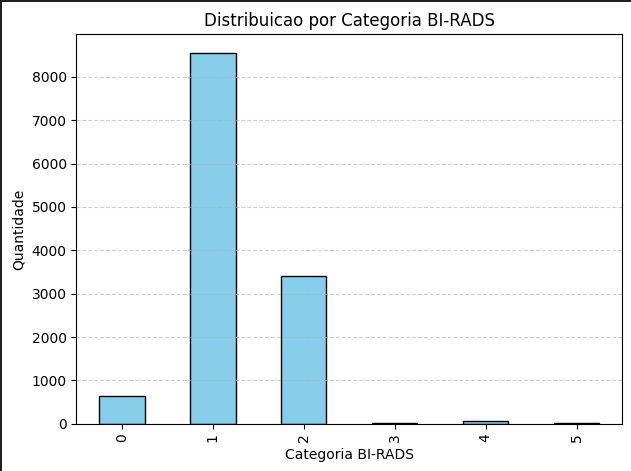
\includegraphics[width=3.5in]{figs/GRAPH.png}
\caption{}
\label{fig:graph}
\end{figure}

Para a avaliação do modelo MedGemma 4B-IT, utilizamos um conjunto real de dados composto por mamografias digitais e seus laudos clínicos associados. As imagens foram obtidas em formato padrão DICOM e convertidos para PNG. Os laudos em PDF foram extraídos os textos identificando qual mama pertence a imagem. Todos os dados foram anonimizados para preservar a privacidade dos pacientes. Os dados foram organizados em um arquivo CSV contendo os caminhos das imagens e as respectivas categorias de achados clínicos.

.Fig~\ref{fig:graph} Distirbuição das categorias BI-RADS O Autor (2025).
\begin{table}[!h]
\renewcommand{\arraystretch}{1.3}
\caption{Distribuição das imagens por categoria BI-RADS}
\label{table:distribuicao_birads}
\centering
\begin{tabular}{|c|c|}
\hline
\textbf{Categoria BI-RADS} & \textbf{Número de Imagens} \\
\hline
0 & 639 \\
\hline
1 & 8.551 \\
\hline
2 & 3.402 \\
\hline
3 & 18 \\
\hline
4 & 63 \\
\hline
5 & 26 \\
\hline
6 & 0 (sem amostras na coleção) \\
\hline
\end{tabular}
\end{table}

Para fins de avaliação qualitativa, foram selecionados aleatoriamente cinco imagens pertencentes às categorias BI-RADS disponíveis, totalizando 30 imagens representativas da coleção.
\begin{table}[!h]
\renewcommand{\arraystretch}{1.3}
\caption{Classificação BI-RADS — Categoria 0}
\label{table:birads_categoria0}
\centering
\begin{tabular}{|c|l|p{2.5cm}|}
\hline
\textbf{Imagem} & \textbf{Categoria Real} & \textbf{Resposta MedGEMMA} \\
\hline
\texttt{32905\_32105\_5\_MLOD.png} & Categoria 0 & Categoria 4 \\
\hline
\texttt{32934\_32134\_1\_CCD.png} & Categoria 0 & Categoria 4 \\
\hline
\texttt{33078\_32286\_1\_CCD.png} & Categoria 0 & Categoria 4 \\
\hline
\texttt{33273\_32499\_1\_CCD.png} & Categoria 0 & Categoria 4 \\
\hline
\texttt{65\_33070\_1\_CCD.png} & Categoria 0 & Categoria 4 \\
\hline
\end{tabular}

\vspace{0.2cm}
\small \textbf{Fonte:} O autor (2025)
\end{table}
A Tabela~\ref{table:birads_categoria0} apresenta a comparação entre as categorias reais de mamografias classificadas como BI-RADS 0 (inconclusivas) e as respostas dornecedias pelo modelo MedGemma. Observa-se que, em todos os casos avaliados, o modelo classificou as imagens como BI-RADS 4, que indica lesões suspeitas e que necessitam de investigação adicional.



\begin{figure}[!h]
\centering
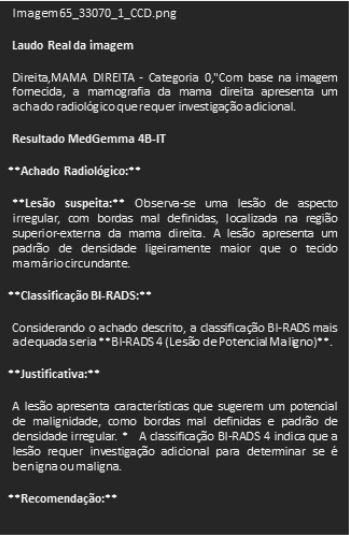
\includegraphics[width=2.5in]{figs/laudo001.png}
\caption{Quadro I}
\label{fig:q1}
\end{figure}


A figura~\ref{fig:q1} apresenta a resposta fornecida pelo modelo MedGemma 4B-IT para a imagem \texttt{65\_33070\_1\_CCD.png}, originalmente classificada como BI-RADS 0 (inconclusiva), demonstra a capacidade do modelo em interpretar achados visuais complexos e atribuir uma classificação baseada em evidências radiológicas. O modelo identificou uma lesão de aspecto irregular, com bordas mal definidas e densidade alterada, localizada na região superior-externa da mama direita, características frequentemente associadas a potencial malignidade. Com base nessa análise, o MedGEMMA classificou o exame como BI-RADS 4, indicando suspeita de malignidade e recomendando investigação diagnóstica adicional, como ultrassonografia ou biópsia. Essa resposta evidencia o funcionamento do modelo ao associar descrições visuais a categorias clínicas, e mostra como, mesmo em casos classificados como inconclusivos por especialistas humanos, a IA pode fornecer uma hipótese diagnóstica mais direcionada o que pode ser útil como suporte, embora nunca substitua a avaliação médica final. 


\begin{table}[!h]
\renewcommand{\arraystretch}{1.3}
\caption{Classificação BI-RADS — Categoria 1}
\label{table:birads_categoria1}
\centering
\begin{tabular}{|c|l|p{2.5cm}|}
\hline
\textbf{Imagem} & \textbf{Categoria Real} & \textbf{Resposta MedGEMMA} \\
\hline
\texttt{68\_33273\_5\_MLOE.png} & Categoria 1 & Categoria 4 \\
\hline
\texttt{1016\_32097\_2\_CCD.png} & Categoria 1 & Categoria 1 \\
\hline
\texttt{2099\_33324\_3\_MLOD.png} & Categoria 1 & Categoria 4 \\
\hline
\texttt{7867\_33891\_1\_CCD.png} & Categoria 1 & Categoria 1 \\
\hline
\texttt{65\_33070\_1\_CCD.png} & Categoria 1 & Categoria 4 \\
\hline
\end{tabular}

\vspace{0.2cm}
\small \textbf{Fonte:} O autor (2025)
\end{table}

A Tabela~\ref{table:birads_categoria1} mostra que, entre as cinco imagens da Categoria Real BI-RADS 1 (exame normal), o modelo MedGEMMA acertou apenas duas, enquanto classificou erroneamente três como BI-RADS 4, indicando suspeita de malignidade. O modelo pode estar superestimando o risco, gerando falsos positivos que podem levar a investigações desnecessárias. 

\begin{table}[!h]
\renewcommand{\arraystretch}{1.3}
\caption{Classificação BI-RADS — Categoria 2}
\label{table:birads_categoria2}
\centering
\begin{tabular}{|c|l|p{2.5cm}|}
\hline
\textbf{Imagem} & \textbf{Categoria Real} & \textbf{Resposta MedGEMMA} \\
\hline
\texttt{65\_33070\_5\_MLOE.png} & Categoria 2 & Categoria 1 \\
\hline
\texttt{943\_32148\_1\_CCD.png} & Categoria 2 & Categoria 4 \\
\hline
\texttt{6779\_33756\_3\_MLOD.png} & Categoria 2 & Categoria 4 \\
\hline
\texttt{32873\_32066\_1\_CCD.png} & Categoria 2 & Categoria 1 \\
\hline
\texttt{32959\_32162\_4\_MLOE.png} & Categoria 2 & Categoria 4 \\
\hline
\end{tabular}

\vspace{0.2cm}
\small \textbf{Fonte:} O autor (2025)
\end{table}
A Tabela~\ref{table:birads_categoria2} o modelo MedGEMMA não conseguiu identificar corretamente nenhum dos casos classificados clinicamente como Categoria 2 do sistema BI-RADS, que representa achados benignos. Reforçar o treinamento com mais exemplos representativos de Categoria 2, capturando variações de lesões benignas e calcificações. 
Ajustar a sensibilidade do classificador para reduzir falsos positivos (superestimações).

\begin{table}[!h]
\renewcommand{\arraystretch}{1.3}
\caption{Classificação BI-RADS — Categoria 3}
\label{table:birads_categoria3}
\centering
\begin{tabular}{|c|l|p{2.5cm}|}
\hline
\textbf{Imagem} & \textbf{Categoria Real} & \textbf{Resposta MedGEMMA} \\
\hline
\texttt{3103\_33104\_2\_CCD.png} & Categoria 3 & Categoria 3 \\
\hline
\texttt{32883\_32077\_3\_MLOD.png} & Categoria 3 & Categoria 4 \\
\hline
\texttt{33751\_33001\_1\_CCD.png} & Categoria 3 & Categoria 2 \\
\hline
\texttt{34648\_33938\_2\_CCE.png} & Categoria 3 & Categoria 4 \\
\hline
\texttt{34648\_33938\_4\_MLOE.png} & Categoria 3 & Categoria 4 \\
\hline
\end{tabular}

\vspace{0.2cm}
\small \textbf{Fonte:} O autor (2025)
\end{table}
Na Tabela~\ref{table:birads_categoria3} observa-se que, embora o modelo MedGEMMA tenha atribuído corretamente a categoria BI-RADS 3 para a imagem \texttt{3103\_33104\_2\_CCD.png}. Para as demais, houve erros importantes.  


\begin{figure}[!h]
\centering
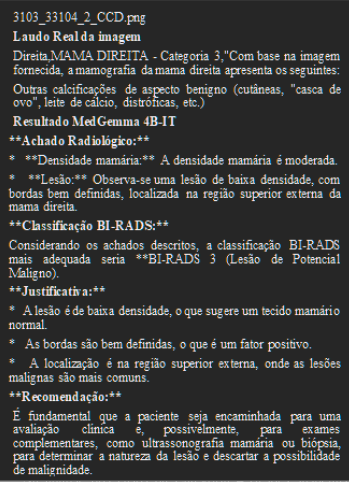
\includegraphics[width=2.5in]{figs/laudo002.png}
\caption{Quadro II}
\label{fig:q2}
\end{figure}


\begin{table}[!h]
\renewcommand{\arraystretch}{1.3}
\caption{Classificação BI-RADS — Categoria 4}
\label{table:birads_categoria4}
\centering
\small
\begin{tabular}{|p{4.8cm}|p{1.5cm}|p{1.7cm}|}
\hline
\textbf{Imagem} & \textbf{Categoria Real} & \textbf{Resposta MedGEMMA} \\
\hline
\texttt{12116\_32829\_1\_CCD.png} & Categoria 4 & Categoria 4 \\
\hline
\texttt{33314\_32543\_1\_CCD.png} & Categoria 4 & Categoria 1 \\
\hline
\texttt{33564\_32805\_1\_CCD.png} & Categoria 4 & Categoria 2 \\
\hline
\texttt{33593\_32835\_4\_MLOE.png} & Categoria 4 & Categoria 1 \\
\hline
\texttt{240408153635\_\ldots\_1\_CCD.png} & Categoria 4 & Categoria 4 \\
\hline
\end{tabular}
\end{table}


\vspace{0.2cm}
\small \textbf{Fonte:} O autor (2025)
\end{table}


Na análise dos casos da Categoria 4 (lesões suspeitas) (Tabela~\ref{table:birads_categoria4}), o modelo MedGEMMA classificou corretamente 2 de 5 imagens como BI-RADS 4, correspondendo à categoria real. 
\begin{table}[H]
\centering
\caption{Classificação BI-RADS Categoria 5}
\begin{tabular}{|c|l|p{2.5cm}|}
\hline
\textbf{Imagem} & \textbf{Categoria Real} & \textbf{Resposta MedGEMMA} \\
\hline
\texttt{1400\_32156\_2\_CCE.png} & Categoria 5 & Categoria 4 \\
\texttt{32927\_32126\_2\_CCE.png} & Categoria 5 & Categoria 4 \\
\texttt{33437\_32676\_1\_CCD.png} & Categoria 5 & Categoria 4 \\
\texttt{33533\_32777\_2\_CCE.png} & Categoria 5 & Categoria 1 \\
\texttt{34402\_33678\_2\_CCE.png} & Categoria 5 & Categoria 1 \\
\hline
\end{tabular}
\label{tab:birads5}
\end{table}

A Categoria BI-RADS 5 representa um alto risco de malignidade (>95\%), sendo essencial que o modelo identifique corretamente tais casos para permitir intervenção médica imediata. No entanto, ao analisar as 5 imagens rotuladas como Categoria Real 5, o modelo MedGEMMA não conseguiu classificar corretamente nenhuma delas como BI-RADS 5. 

Apesar dos resultados inicias apresentam uma acurrácia insatisfatória o MedGemma na classificação das categorias BI-RADS, é importane destacar que o modelo não passou por um processo de ajuste fino (fine-tuning) específico para mamografia. Para este estudo foi considerado apenas o modelo pré treinado. O fine-tuning com um conjunto de dados balanceado, rotulado por especialistas e representativo das diversas variações clínicas pode ser uma etapa fundamental para melhorar significativamente o desempenho. 

\section{CONCLUSÃO}

O estudo destaca os desfios enfrentados por modelos multimodais como o MedGemma para tarefas críticas de classificação de imagens médicas, embora evidenciando a limitação em termos de acurácia, os resultados atuais estejam a baixo do desejado para aplicação médica segura, eles apotam o potencial promissor de aprimoramento por meio do fine-tuning.  

Como trabalhos futuros, propõe-se a realização de fine-tuning supervisionado utilizando um conjunto de dados com quantidade suficiente de imagens representativas e balanceadas entre as categorias BI-RADS, acompanhadas de seus respectivos laudos clínicos. Essa abordagem permite especializar o modelo para o domínio da mamografia, reduzindo erros e ampliando a sensibilidade e a confiabilidade do sistema. Além disso, recomenda-se a aplicação de métricas por classe, análise de erro e a integração de validação com especialistas, de modo a desenvolver soluções de apoio ao diagnóstico mais robustas, seguras e clinicamente relevantes. 



\bibliographystyle{IEEEtran}
\bibliography{bibliografia}

\end{document}